\documentclass[a4paper,11pt]{article}
\usepackage{amssymb}
\usepackage{mathbbold}
\usepackage{latexsym}
\usepackage{amsmath}
\usepackage{url}
\usepackage{graphicx}
\usepackage{amsthm}
\parindent=0in
\author{Bi Ran(U087272L)}
\title{Hand Written Digit Recognition and Its Improvement}
\frenchspacing

\begin{document}
\maketitle
\begin{abstract}
Handwritten digits recognition is a classic problem of machine learning. The objective is to recognize images of single handwritten digits(0-9). This paper will apply C4.5 decision tree, boosted C4.5, and support vector machine(SVM) on this problem, compare their performance, and finally propose a method to improvement the classification accuracy by adding attributes into data set.
\end{abstract}
\section{Introduction}
Handwritten digit recognition recognition is a classification problem. The performance of classification algorithm heavily depends on properties of data set.
In this paper, Semeion Handwritten Digit Data Set is used for training and testing. The first part of the paper will show the result of C4.5, boosted C4.5 and SVM algorithms.
It will be shown that the performance of decision tree is poor by itself, but much better after being boosted; SVM gives the best performance in these algorithms. Parameter search is applied to achieve relatively good performance for C4.5 and SVM.
The second part will introduce a method to improve accuracy of classifiers by adding extra features into data set. It will be shown that performances of all three algorithms have significant improvement on the modified data set, and SVM with RBF kernel achieves error rate of 3.7037\%.
\section{Background and Motivation}
Handwritten digit recognition has important usage such as recognizing zip code, online recognition on computer tablets. Algorithms like support vector machine and multi layer perceptron are commonly used on this problem, and impressive result has been achieved. Lenet and its boosted version managed to get error rate less than 1\% on MNIST data set\cite{Kussul_improvedmethod}. SVM also gives one of the lowest error rate among many classification algorithms.
\section{Data set}
Semeion Handwritten Digit Data Set(\url{http://archive.ics.uci.edu/ml/datasets/Semeion+Handwritten+Digit}) is used in this paper. The data set was created by Tactile Srl, Brescia, Italy (\url{http://www.tattile.it}) and donated in 1994 to Semeion Research Center of Sciences of Communication, Rome, Italy (\url{http://www.semeion.it}), for machine learning research.
1593 handwritten digits from around 80 persons were scanned, stretched in a rectangular box 16x16 in a gray scale of 256 values.Then each pixel of each image was scaled into a boolean (1/0) value using a fixed threshold. This data set contains no missing values.
Each person wrote on a paper all the digits from 0 to 9, twice. The commitment was to write the digit the first time in the normal way (Figure 1) and the second time in a fast way (Figure 2).
\begin{figure}
\centering
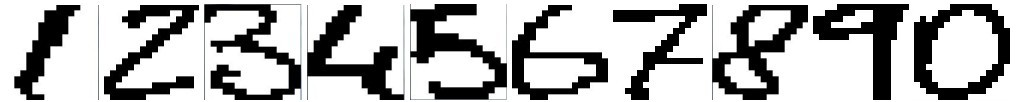
\includegraphics[width=1.0\textwidth]{clear}
\caption{written in normal way}
\end{figure}

\begin{figure}
\centering
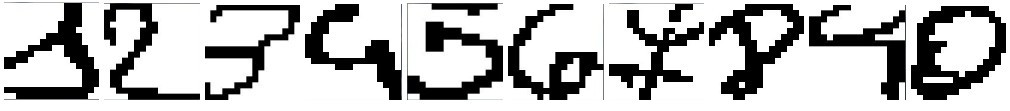
\includegraphics[width=1.0\textwidth]{unclear}
\caption{written in fast way}
\end{figure}
This data set consists of 1593 records (rows) and 256 attributes (columns).
Each record represents a handwritten digit, originally scanned with a resolution of 256 grays scale.
Each pixel of the each original scanned image was first stretched, and after scaled between 0 and 1 (setting to 0 every pixel whose value was under the value 127 of the grey scale (127 included) and setting to 1 each pixel whose original value in the grey scale was over 127).
Finally, each binary image was scaled again into a 16x16 square box (the final 256 binary attributes).\\
The order of the examples in the data set is shuffled before training and testing, because the label distribution of the original data set is not random.
\section{Evaluation}

The data set contains 1593 instances, which not very big. In this paper, cross validation is used to perform testing. \\
By applying cross validation on different fold number using C4.5 algorithm(with default parameters in WEKA), we observe that the error rate almost keeps still after 8 fold. 8-folds cross validation is very likely to provide accurate estimation of the real error rate on unseen data. In this paper, we apply 10-folds cross validation on the whole Semeion Handwritten Digit Data Set for testing, and compare the error rates of different algorithms.\\
\emph{WEKA}(\url{http://www.cs.waikato.ac.nz/ml/weka/}) is used for training and testing of C4.5 and boosted C4.5 algorithm, and \emph{libsvm} package(\url{http://www.csie.ntu.edu.tw/~cjlin/libsvm/}) implemented by Chih-Chung Chang and Chih-Jen Lin is used for training and testing SVM in this paper.\\

\vspace{0.5cm}
\begin{tabular}{c c}
Fold Number & Error Rate\\
\hline \hline
2  &29.0019\%\\
4  &25.6121\%\\
6  &24.231 \%\\
8  & 24.6704\%\\
10 & 23.9799\%\\
12 & 24.8588\%\\
14 & 24.5449\%\\
\end{tabular}
\vspace{0.5cm}\\
\section{Testing}
\subsection{C4.5}
Decision tree is a popular algorithm in data mining and machine learning. There are many decision tree algorithms. We only apply C4.5 in this paper. C4.5 is an improved version of ID3 decision tree. It follows a simple inductive bias, which is ``smaller trees are preferred''. This inductive bias is motivated by Occan's Razor principle, and it works well in practice.\\
To further simplify the decision tree to avoid over fitting problem, C4.5 perform pruning to limit the size of the tree. To achieve good performance, we perform parameter search on two parameters: $C$ and $minObj$. \\
$C$ is confident factor, which is a probability threshold of the probability of the actual error rate being worse than the pessimistic estimation\cite{Morgan.Kaufmann}. The pessimistic estimation of the error rate for each subtree is used when do the subtree replacement and subtree raising pruning in C4.5 algorithm. Smaller confidence factor implies more pessimistic estimation, which will cause more drastic pruning.\\
The $minObj$ variable limit the minimum number of examples each leaf could have. This constrain can help reduce the size of the tree, thus makes the tree more robust to the effect of noise.
\vspace{0.5cm}\\
\begin{tabular}{c|c c c c}
C$\backslash$ minObj	&1		&2		&3		&4\\
\hline \hline
1e-3 	&24.6077 \%	&24.3566 \%	&24.1682 \%	 &24.6704 \%\\
1e-2	&24.4193 \%	 &24.4821 \%	&24.231  \%	 &24.5449 \%\\
1e-1	&24.6077 \%	&24.231  \%	&24.231  \%	 &24.6077 \%\\
0.5 &24.2938 \%     &24.0427 \% &24.1055 \%  &24.8588 \%\\
1	&24.6077 \%	&23.7916 \%	&24.1682 \%	 &24.796  \%\\
\end{tabular}
\vspace{0.5cm}\\
The result in the table above shows that he error rate of C4.5 algorithm is lowest when $C=1$ and $minObj=2$, which gives error rate of 23.7916\%. The differences between error rates are very small, which implies that pruning does not help much in this data set.\\
This result is very poor compared to many other popular algorithms like support vector machine(will see it later). There are some possible reasons:\\
\begin{enumerate}
\item[1] This is because the limitation of decision tree algorithm itself. The problem of learning optimal decision tree is NP-complete\cite{DT_NPC}. C4.5 use a greedy algorithm, which does not guarantee to find the optimal decision tree.\\
\item[2] Although decision tree can estimate any discrete functions, it is difficult to learn certain functions like OXR, because the minimal decision tree for XOR requires a full binary tree with each leaf for one instance, and it is hard to find ``small'' trees to estimate XOR well.
\item[3] C4.5 decision tree supports multi-class classification problem. More classes would result in larger trees. For example, if there are $N$ classes, and each attribute is binary. Since each leaf can only represent one class, the height of the tree must be larger than $log_2(N)$. Larger tree would contradict to Occan's Razor principle. Thus, C4.5 may not perform well in multi-class classification problems.
\end{enumerate}
We can overcome the 3rd effect mentioned above by converting multi-class classification problem into two-class classification problem.\\
Several possible methods can be used for this conversion. We only consider ``pairwise'' method in this paper. Pairwise method train $C_N^2$ classifiers for each pair of classes($N$ is the number of classes). When classifying a new instance, each classifier classifies the new instance, and vote for the class based on their results. The class with the highest vote is considered as the classification result. If draw happens, randomly choose one of the classes with the highest vote.\\
Weka itself does not support this conversion, so I wrote a separate program based on WEKA's library to do this test.
Source code is available at \url{http://code.google.com/p/cs2306-machine-learning/source/browse/trunk/J48Test.java}\\
\vspace{0.5cm}
\begin{tabular}{c c}
Algorithm	& Error rate\\
\hline \hline
original C4.5	& 23.7916\%\\
pairwise C4.5	& 15.5345\%\\
\end{tabular}
\vspace{0.5cm}\\
We can see from the table that pairwise C4.5 performs much better than original C4.5. This is because in pairwise C4.5, although there are more decision trees, the size of each tree is small(about 20 on average). However, the size of the tree for the original C4.5 is 293(use full data set to train). Thus, pairwise C4.5 performs better, since small trees are more likely to generalize well on unseen data.
\subsection{Boosting}
Boosting is an algorithm which aims to boost week classifier into a strong classifier. The boosting algorithm used here is AdaBoosting M1, which is
generalization of AdaBoosting algorithm on multiple class classification problem.\\
The boosting algorithm constructs the classifier by several iterations, each iteration obtains a classifier by a weighted data set, and the output of the final classifier is obtained by weighted sum of the results of all classifiers. After each iteration, data set is reweighted, and misclassified instances has a larger weight so that they are paid more attention on in the next iteration. The weight of each classifier is decided by their accuracy. Boosting works well with decision tree in practice, and it often does not suffer from over fitting problem.\\
Following result is obtained by applying boosting on C4.5 algorithm($C=1$ and $minObj=2$) with different number of iterations.\\
\vspace{0.5cm}
\begin{tabular}{c c}
Number of Iterations	& Error rate\\
\hline \hline
	2		& 23.7916\%\\
	4		& 17.7024\%\\
	8		& 13.4965\%\\
	16		& 9.6673\%\\
    32      & 7.7841\%\\
    64      & 6.6541\%\\
\end{tabular}
\vspace{0.5cm}\\
From the table, we can see that the error rate drops rapidly when the number of iteration grows. Although higher accuracy can be achieved by further increase the number of iterations, the error rate would stop decreasing or start to increase(over fitting) at last.\\
Boosting algorithm constructs a classifier by combining several classifiers, which intuitively increase the complexity of the classifier. However, according to Occan's Razor principle, simpler classifiers tend to generalize better on unseen data. Boosting algorithm seems a contradict with Occan's Razor principle.\\
One possible explanation is that the complexity of classifier is not measured by the number of classifiers, but by the ``margin'' of the classifier.
In Boosting algorithm, each classifier vote to a class by its weight, and the class with the highest weight is the result of classification. The margin of an example is defined by the difference between weight of correct class, and the sum of all weights of incorrect class. The larger the margin is , the more confident the classification for this instance is. The boosting algorithm tend to maximize margin of instances, and convergence with some large margin distribution\cite{boosting}.
\subsection{Support Vector Machine}
Support vector machine can be seen as a generalized version of linear classifier. To classify data set which is not linear separatable, SVM maps each example into a higher dimensional feature space, and find a hyper plane, which separate different classes. The margin of hyper plane is defined as the distance of the plane to the closest example. Hyper plane with large margin is preferred. All calculation of feature vector with high dimension can be done by kernel function, which makes training and testing more efficient. Although new kernel functions are being purposed by researchers, four basic kernels are most popular:\cite{SVM}
\begin{itemize}
\item linear: $K(x_i,x_j)=x_i^Tx_j$\\
\item polynomial: $K(x_i,x_j)=(\gamma x_i^Tx_j+r)^d$, $\gamma >0$\\
\item radial basis function (RBF): $K(x_i,x_j)=\exp(-\gamma + \|x_i-x_j\|^2)$, $\gamma > 0$\\
\item sigmoid: $K(x_i,x_j)=tanh(\gamma x_i^Tx_j+r)$\\
\end{itemize}
According to Keerthi and Lin (2003) and (Lin and Lin, 2003), linear kernel is a special case of RBF kernel, and sigmoid kernel behaves like RBF kernel with certain parameters. So in this paper, we only use RBF kernels.\\
There are many kinds of SVMs based on different error function it aims to minimize. In this paper, we simply use C-svm, which minimize function:
 subject to:$$\frac{1}{2}\|\vec{\beta}\|^2+C\sum_{i=1}^n \xi_i$$
 subject to:$$y_i(\vec{\beta}.\vec{x_i}+\beta{0})\geq 1-\xi_i$$$$\forall i, \xi_i\geq 0$$

For C-SVM using RBF kernel, $C$ and $\gamma$ are adjustable parameters. To find the optimal parameter, we can use grid-search proposed in \cite{SVM}: construct exponential growth sequence of $C$ and $\gamma$, and use a coarse grid search to find a ``better'' region, and apply grid search on that region to find more accurate parameters. Tools provided in \emph{libsvm} package are used to perform the model selection automatically.\\
As shown in Figure 3, the SVM tends to perform best when $C=2.0$ and $\gamma=0.0078125$, and the error rate is 4.2059\%.

\begin{figure}
\centering
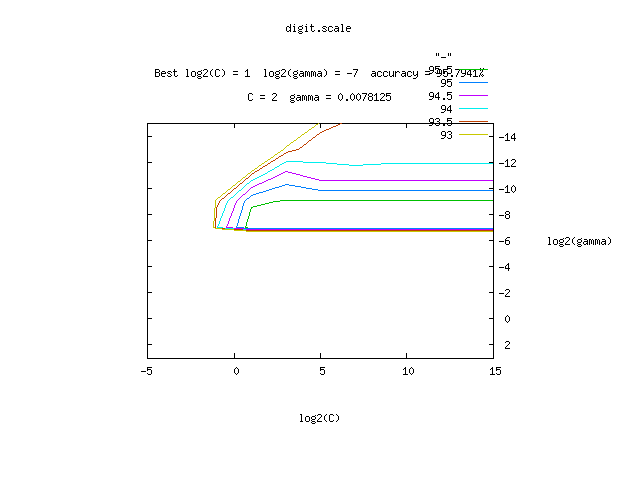
\includegraphics[width=1.0\textwidth]{digit}
\caption{grid search on $C,\gamma$}
\end{figure}

\section{Improvement}
\subsection{Motivation}
One observation is that for decision tree and SVM, the order of attributes is not important for training and classification. In other word, if some fixed permutation is applied on the attributes of each example in the data set, then decision tree and SVM will generate the same model as the model generated by original data set.\\
However, the position of pixel is important in the process of human being recognizing a hand written digit. If the pixel of an image randomly re arranged, a human is very unlikely to recognize what's in the image. This motivate the preprocessing of data, which can make use of position information of pixels. In this paper, we try to add some attributes derived by position information.
\subsection{Adding Features}
To provide information about the position of pixels, we choose to add $16$ extra attributes $r[16]$, one for each row, which describes how many ``black segments'' are there in the row. In image of $1$, most of $r[i]$ can be expected to be $1$, and some can be $2$, depends on the way of writing. In image of 0, most $r[i]$ can be expected to be 2.
Similarly, 16 more attributes $c[16]$ is added for each column, which means the number of `black segments'' in each column.
The variance of the number of black pixels in each row, and the variance of the number of black pixels in each column are also added into each example.

34 extra features are added into each examples.The modified data set has 290 features for each example.
\subsection{Testing}
\vspace{0.5cm}
\begin{tabular}{c c c}
Algorithm		&	Original Data	&Modified Data\\
\hline \hline
C4.5($C=1, minObj=2$)           &23.7916\%		& 18.5813\%\\
Boosted C4.5(32 iterations)	    &7.7841\%		& 4.5198\%\\
Boosted C4.5(64 iterations)	    &6.6541\%		& 4.457\%\\
SVM($C=2, \gamma=0.0078125$)	&4.2059\%       & 3.2643\%\\
\end{tabular}
\vspace{0.5cm}\\
In the testing, From the result, we can see improvements on all algorithms are significant. All algorithm's error rate on modified data drop down to the $\frac{3}{4}$ of the original data.\\
Although decision tree and SVM use completely different way to look for target hypothesis, attributes which contains position information of pixels helps both of them improve accuracy. It can be expected that adding more features derived by position information of pixels could further improve the accuracy, and the improvement may be observed on other algorithms. This technique can be expected to work on general image classification problem whose data set only contains information about pixels color of images.

\section{Conclusion}
By applying several machine learning algorithms on Semeion Handwritten Digit Data Set, we can observe that C4.5 algorithm performs poorly even after choosing appropriate parameters, while boosted C4.5 has a much better performance. C-SVM with RBF kernel managed to reach 4.2059\% error rate after parameter search. By adding extra information into the data set, the error rate for all these algorithm drops down to about $3/4$ of their original error rate.

\bibliographystyle{h-physrev3}
\bibliography{ref}
\end{document}
